\documentclass[a4paper,12pt]{article}
\usepackage{listings}
\usepackage{amsmath}
\usepackage{amssymb}
\usepackage{graphicx}

\author{E. Routledge}
\date{01 Nov 2022}
\title{Sudoku and Other Related Problems}

\begin{document}
\lstset{language=Python}
\maketitle

% ~~~~~~~~~~~~~~~~~~~~~~~~~~~~~~~~~~~~~~~~~~~~~~~~~~~~~~~~~~~~~~~~~~~~~~~~~~~~~~~~~~~~~~~~~~~~ %
\section{Introduction}
		Sudoku is a simple logic game, in the standard $9 \times 9$ (or $3 \times 3 \times 3 \times 3$) 
		one must complete the grid such that every row, column and box contains the numbers 1 to 9, that is all,
		yet it is filled with mathematics. Through sudoku we can explore the connections between various areas of maths: complexity theory, graph theory, group theory and information theory.
	\subsection{History}
	
	\subsection{Defining Sudoku Notation}
	
	\textbf{Def$^n$}: A valid sudoku puzzle is a function $ S: i,j \rightarrow x$ for values i,j $\in \{1,...,D^2\}$ and $x \in \{0,...,D^2\}$ satisfying the following:
\begin{itemize}
	\item{for all $a,b,c$  $\in \{1,...,D^2\}$ with $S(a,b)\neq$ 0 and $S(a,c)\neq$ 0, then $ S(a,b)\neq$ S(a,c) }
	\item{for all $a,b,c$  $\in \{1,...,D^2\}$ with $S(a,b)\neq$ 0 and$ S(c,b)\neq$ 0, then $S(a,b)\neq$ S(c,b) }
	\item{for all $ a,b,c,d $ $\in \{1,...,D^2\}$ with $a mod D = c mod D$, $b mod D  =  d mod D$, $S(a,b)\neq$ 0 and $S(c,d) \neq$ 0, then $S(a,b)\neq S(a,c)$ }
\end{itemize}
\textbf{Def$^n$}: A completed sudoku puzzle is a function $ S: i,j \rightarrow x$ as above but with the added condition that $x \neq 0$.

% ~~~~~~~~~~~~~~~~~~~~~~~~~~~~~~~~~~~~~~~~~~~~~~~~~~~~~~~~~~~~~~~~~~~~~~~~~~~~~~~~~~~~~~~~~~~~ %
\section{Classic solving techniques}

\textbf{Def$^n$}: A forced cell is a value pair $(a,b)$ such that $S(a,b)$ can only be a single value call this $x$ as $\{1,...,D^2\}/\{x\}$ are already present in $S(a,j)$ for $j \in\{1,...,D^2\}/\{b\}$ or $S(i,b)$ for $i \in\{1,...,D^2\}/\{a\}$ or $S(i,j)$ where $a mod D = i mod D$ and $b mod D  =  j mod D$.

define x wing
define y wing
% ~~~~~~~~~~~~~~~~~~~~~~~~~~~~~~~~~~~~~~~~~~~~~~~~~~~~~~~~~~~~~~~~~~~~~~~~~~~~~~~~~~~~~~~~~~~~ %
\section{Sudoku is Hard}

Sudoku can be described in a single rule but it is in fact a hard problem to solve. Instances of the puzzle requiring complex x wing and y wing strategies are not what makes the puzzle hard to solve, it is hardness through a provable, computational lense for which this section cares. 
		
\subsection{Computational Complexity an Introduction}
	
	 \textit{TO COMPLETE: DEFINE BIG O NOTATION}

	\textit{KARP REDUCTION}
	 
\textbf{What is NP completeness?}
We care about decision problems, these are problems that given an input  produce a 'yes' or 'no' answer. We will discuss three sets of these problems: 
\begin{itemize}
	\item{P is the the class of problems that can be solved in polynomial time (if the input is order n then the program halts in order $n^2$ steps) by a Turing machine;} 
	\item{NP is the class of problems that can be verified in polynomial time and solved in polynomial time by a non-deterministic Turing machine;} 
	\item{the NP-complete set has problems that any NP problem can be reduced to in polynomial time.} 
\end{itemize}

NP problems are hard as it is assumed they cannot be solved in polynomial time ($P \neq NP$) and are therefore infeesible for large inputs. We can only assume that $P\neq NP$ as this problem is yet to be proven, it is in fact one of the Millennium Prize problems.

\begin{figure}[h!]
	\begin{center}
		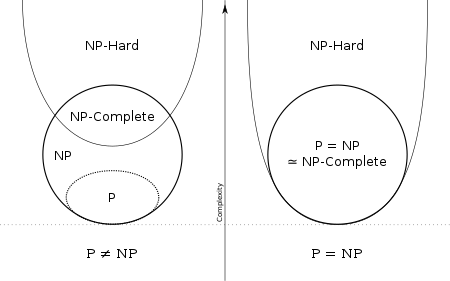
\includegraphics[width=60mm]{P_np.svg}
	\end{center}
	\caption{P, NP, NP-complete \& NP-hard sets \cite{P_NP_Figure}}
\end{figure}

\textbf{How to prove NP completeness generally?}
Call the problem we wish to prove is NP-complete $x$. First show there exists a verifier for $x$ with a polynomial or less runtime, this is a algorithm that decides if a proposed solution to problem $x$  is correct. Then reduce a known NP-complete problem call this $y$ to $x$, one does this by transforming the input of $y$ to the input of $x$ in polynomial time. If there exists a polynomial time algorithm to solve $x$ we could solve$y$ in polynomial time too, this implies P=NP, a contradiction. Therefore a polynomial time algorithm does not exist for $x$.

\textbf{Our base NP-complete problem.} If, as the above suggests, we require a NP-complete problem to prove a problem is NP-complete then we seem to have reached a paradox. Luckily we have the Cook-Levin Theorem.

\textit{Cook-Levin Theorem:} SAT is NP-Complete
	
\textit{Proof:}	 \textit{TO COMPLETE: CITE }

\textbf{Def$^n$}: SAT is the following decision problem. Given a set of boolean variables $B$ and a collection of clauses $C$ does a valid truth assignment exist that satisfies $C$?

We now have a NP-complete problem to reduce other problems to.

\textbf{More on polynomial time and big O notation.} 

\subsection{Verification is Easy}
Verificaiton decision problem, "is the sudoku puzzle complete?":

		\begin{equation}
			\Psi(S(,)) = \begin{cases}	
				\text{True if the puzzle is complete} \\
				\text{False if the puzzle is not complete}.
			\end{cases}
		\end{equation}

There exists an algorithm to do this in polynomial time with respect to the dimensions of the grid. 
\begin{enumerate}
\item For each row in the grid check there exists no repeated numbers. $O(n^2)$
\item For each column in the grid check there exists no repeated numbers. $O(n^2)$
\item For each box in the grid check there exists no repeated numbers. $O(n^2)$
\end{enumerate}
If all tests pass return True else return False.
This algorithm has complexity of $O(n^2 + n^2 + n^2) = O(3n^2) = O(n^2)$, this is polynomial and therefore $\Psi(S(,)) \in P$.

	\subsection{Finding a Solution is Hard}
		
Finding a solution to sudoku is NP-complete, let us define the decision problem:

		\begin{equation}
		        \Phi (S(,)) = \begin{cases}
		            \text{True if a completion exists} \\
		            \text{False if a completion does not exist}.
				\end{cases}
		\end{equation}

Our question now is does there exist a function $\Phi$ that when given an instance of the problem will, in polynomial time or less, return True if it can be solved and False otherwise.

\subsubsection{\textbf{\underline{Proof}}}

The \textbf{verifier} is $O(n^2)$, as will be seen in the above subsection 'Validation is Easy'.

Now we need a \textbf{reduction} from sudoku to a known NP-complete problem to prove sudoku is at least as hard. We will be creating a chain of reductions: Sudoku $\geq_p$  Latin Square $\geq_p$  Triangulated Tripartite $\geq_p$  3SAT and then prove 3SAT is NP-complete.

\subsubsection{Sudoku $\geq_p$ Latin Square}

\textbf{Def$^n$}: A valid Latin Square puzzle is a function $L:i,j \rightarrow x$ for values $i,j \in \{1,..,D\} $ and $x \in \{0,...,D\}$ satisfying the following:
\begin{itemize}
\item{for all $a,b,c \in \{1,...,D\}$ with $L(a,b) \neq 0 $ and $L(a,c) \neq 0$ then $L(a,b) \neq L(a,c)$}
\item{for all $a,b,c \in \{1,...,D\}$ with $L(a,b) \neq 0 $ and $L(c,b) \neq 0$ then $L(a,b) \neq L(c,b)$}
\end{itemize}
It is complete or solved if for all $i,j \in \{1,...,D\}$, $L(i,j) \neq 0$.

By observation we see this is a superset of the sudoku puzzle, we just add the restrictions that the dimension must be a square number and also add the third property of the sudoku puzzle defintion.

\textit{What is the Latin Square decision problem?} Given a latin square puzzle $L(,)$, can the function be augmented, by changing only the value of the function for value pairs $i,j$ that previously gave $L(i,j) =0$, to get a complete latin square puzzle?


\textit{Proof idea:} We must reduce a given latin square grid of size $D \times D$ to a sudoku grid size $D^2 \times D^2$ that is solvable iff the Latin square is. 

\textbf{Lemma:} Let $S_l$ be a Sudoku problem with the following construction 
\begin{equation}
	S_l(i,j) =\begin{cases}
0 \qquad\qquad\qquad\qquad\qquad\qquad\text{when } (i,j) \in L_s \\ 
((i-1 \text{ mod } n)n + \left\lfloor{i-1/n}\right\rfloor+j-1)\text{ mod } n^2 +1 \quad\text{otherwise}
\end{cases}
\end{equation}
where $L_s=\{(i,j)| \left\lfloor{i-1/n}\right\rfloor=0 \text{ and }(j \text{ mod }n)=1\}$. Then  there exists an augmentation $S_l'$ to complete the sudoku puzzle if and only if the square $L$ such that $L(i,j/n)=S_l'(i,j)-1/n+1$ for all $(i,j) \in L_s$ is a Latin square.

\textit{Proof:}

First we must show $S_l(i,j)=((i-1 \text{ mod } n)n + \left\lfloor{i-1/n}\right\rfloor+j-1)\text{ mod } n^2 +1$ forms a complete and valid sudoku puzzle.

When $i=[1,...,n^2]$ then:
\begin{align}
	0&<\left\lfloor{i-1/n}\right\rfloor<n-1\\
	0&<i-1 \text{ mod } n<n-1\\
	0&<(i-1 \text{ mod } n)n + \left\lfloor{i-1/n}\right\rfloor<n^2-n\\
	0&<(i-1 \text{ mod } n)n + \left\lfloor{i-1/n}\right\rfloor+j-1<n^2-1\\
	1&<((i-1 \text{ mod } n)n + \left\lfloor{i-1/n}\right\rfloor+j-1)\text{ mod } n^2 +1<n^2\\
	1&<S_l(i,j)<n^2
\end{align} 
Note $\left\lfloor{i-1/n}\right\rfloor$ gives the row coordinate when indexed at 0 in which the larger box that (i,j) belongs to starts and $i-1 \text{ mod } n$ gives the row within that box when indexed at 0. Therefore $(\left\lfloor{i-1/n}\right\rfloor,i-1 \text{ mod } n)$ will take all value pairs of integers between 0 and $n-1$.

When j is fixed (particular column), assume two cells have the same value, that is $S_l(i,j)=S_l(i',j)$ then
\begin{align}
	(i-1 \text{ mod } n)n + \left\lfloor{i-1/n}\right\rfloor+j-1 &= (i'-1 \text{ mod } n)n + \left\lfloor{i'-1/n}\right\rfloor+j-1\\
	(i-1 \text{ mod } n)n + \left\lfloor{i-1/n}\right\rfloor &= (i'-1 \text{ mod } n)n + \left\lfloor{i'-1/n}\right\rfloor
\end{align}
from the above $i=i'$. No cell on a column has the same value.

When i is fixed (particular column) assume two cells have the same value, that is $S_l(i,j)=S_l(i,j')$ implies $j-1=j'-1 (mod n)$ therefore $j=j'$.

For the third condition fix $\left\lfloor{i-1/n}\right\rfloor$. (i-1 \text{ mod } n,j) takes all value pairs of integers 0 to n-1 so if a cell has the same value as another within the n by n square $S_l(i,j)=S_l(i',j')$ implying $(i-1 \text{ mod } n,j)=(i'-1 \text{ mod } n,j')$ which means $i=i'$ and $j=j'$. Therefore $S_l$ is a valid and complete sudoku puzzle.

Now consider which integers fill the blanks in $L_s$. For $(i,j)\in L_s$, $S_l(i,j)-1= ((i-1 \text{ mod } n)n+j-1)\text{ mod } n^2$ as $j mod n=1$, $j-1modn=0$ therfore $S_l(i,j)-1$ is divisible by n so $S_l-1/n+1$ gives integers between $[1,...,n]$. Therefore $L(i,j) \in [0,...,n]$.

We must validate the Latin square conditions. The row constraint in $S_l$ ensures $S'(i,j)=S'(i,j') \implies j=j'$, $S'(i,j)-1/n+1=S'(i,j')-1/n+1 \implies j=j'$, $L(i,j/n)=S'(i,j'/n) \implies j=j'$  is equivalent to the row constraint of L. The column constraint of $S_l$ is equivalent to the column constraint of L. The small square constraint of $S_l$ is equivalent to the column constraint of L. $\square$

\subsubsection{Latin Square $\geq_p$ Triangulate A Tripartite Graph}

\textbf{Def$^n$}: A graph $G=(V,E)$ is tripartite if a partition $V_1$, $V_2$, $V_3$ exists such that the vertices are split into three sets with no edges between vertices that belong to the same set, i.e for all $(v_i,v_j) \in E\text{ if } v_i \in V_i\text{ then }v_j \not\in V_i $.

\textbf{Def$^n$:} A triangulation T of a graph is a way to divide edges into disjoint subsets $T_i$, each forming a triangle ($T_i=\{(v_{1}, v_{2}),(v_{2}, v_{3}),(v_{3},v_{1})\}$).

If a tripartite graph can be triangulated it must be uniform, that is: every vertex in $V_1$ (or $V_2$ or $V_3$) has the same number of neighbour in $V_2$ and $V_3$ (or the respective sets).

\textit{What is the Triangulated Tripartite decision problem?} Given a graph G that is tripartite (can be split into 3 subgroup, within these subgroups vertices should not share edges) can it be triangulated ?

\textbf{Theorem:} Completing a Latin square with dimensions n by n is equivalent to triangulating a tripartite graph $G= V_1, V_2, V_3$.

\textit{Proof:} 

Observe completing a partial Latin square is equivalent to triangulating tripartite graph, we map the Latin square to this through the following: 
given tripartite graph G=(V,E) label vertices in $V_1$ with distinct lables $\{r_1,...r_n\}$, label vertices in $V_2$ with distinct lables $\{c_1,...c_n\}$ and label vertices in $V_3$ with distinct lables $\{e_1,...r_n\}$. Add edges such that:
\begin{itemize}
\item{If $L(i,j) = 0$ then add the edge $(r_i,c_j)$ }
\item{If for all $i \in [0,...,n]$ and constant j, $L(i,j) \neq k$ then add the edge $(r_i,e_k)$}
\item{If for all $j \in [0,...,n]$ and constant i, $L(i,j) \neq k$ then add the edge $(c_j,e_k)$}
\end{itemize}
This graph has a triangulation iff L(i,j) can be solved.

Let us show every uniform tripartite graph is the above formulation of a Latin square.

Defn: A Latin framework LF for tripartite graph G, size (r,s,t) is a r by s array with values [1,...,t]. With constraints:
\begin{itemize}
\item{Each row/column contain each element only once.}
\item{If $(r_i,c_j)\in E$ then LF(i,j)=empty else LF(i,j)= k $k\in [1,...,t]$}
\item{If $(r_i,e_k)\in E$  then for constant i $LF(i,j)\neq k$}
\item{If $(c_i,e_k)\in E$  then for constant j $LF(i,j)\neq k$}
\end{itemize}
If r=s=t then LF is a latin square which can be completed iff G has a triangle partition.

Lemma: For graph G=(V,E) with |V|=n, there's a Latin framework of (n,n,2n).

Define LF an n by n array. For $(r_i,c_j)\in E$ $LF(i,j)=0$ else $LF(i,j)=1+n+((i+j)mod n)$. LF is a latin framework. $\square$

Lemma: Latin framework L  (r,s,t) for uniform tripartite graph G. R(k) = the number of times k appears in L plus half $|e_k|$. Whenever $R(k)\ge r+s-t$ for $1 \le k \le t$, L can be extended to (r,s+1,t) to give L' in which $R'(k)\ge r + s+1-t$ for all $1\le k \le t$.

\textit{proof of this lemma to be added}

Lemma: Latin framework (r,s,s) can be extended to (s,s,s).

We can transpose the array and do the same as the previous lemma. $\square$

Given a tripartite graph G, if it is not uniform then no triangulation exists, else we apply above to produce a latin framework of size (2n,2n,2n) in polynomial time. This is a Latin square which can be completed iff G has a triangulation. The latin square problem has been reduced to the triangulating a tripartite graph problem. $\square$

\subsubsection{Triangulated Tripartite $\geq_p$ 3SAT}

\textit{What is 3SAT?} With a set of boolean variables $B$ and a collection of clauses $C$, with at most 3 literals (a literal is any $b \in B$ or its negation $\bar{b}$) in each, does a valid truth assignment exist that satisfies $C$?
		\begin{equation}
		        \phi (C,B) = \begin{cases}
		            \text{True if a truth assignment exists} \\
		            \text{False if a truth assignment does not exist}.
				\end{cases}
		\end{equation}
This decision problem is therefore an enforced limitation of SAT as defined in the subsection Computational Complexity an Introduction.

\textit{Proof:}

Describe the special graph $H_{3,p}$.
Show graph constructed is tripartite.



 \textit{TO COMPLETE: UNDERSTAND \cite{tripartite to sat}}

\subsubsection{3SAT is NP-Complete}
%%%%% define clause

\textit{Proof:}

Given a truth assignment $t$ check each clause is satisfied, if all are satisfied return True else False, this algorithm is at most the length of $C$ multiplied by the length of $B$. $O(BC)$ is polynomial, a polynomial verifier exists. 

Given a SAT instance with the input sets of $B$ and $C$. $C$ is in conjunctive normal form (every clause set can be converted to an equivalent set in CNF form \cite{CNF}) such that $\forall c \in C$ and for some $b_1, ... ,b_n \in B$, $c = b_1 \lor b_2 \lor ... \lor b_n$. For each $c \in C$ with more than 3 literals we can transform these to a new set of clauses of length 3. 

For $c = b_1 \lor b_2 \lor ... \lor b_n$ we introduce a new literal: $a_1$ to give $b_1 \lor b_2 \lor a_1$, $\bar{b_1} \lor a_1$, $\bar{b_2} \lor a_1$ and $a_1 \lor b_3 \lor ... \lor b_n$. Then $a_1 \lor b_3 \lor ... \lor b_n$ becomes $b_3 \lor b_4 \lor a_2$, $\bar{b_3} \lor a_2$, $\bar{b_4} \lor a_2$ and $a_1 \lor a_2 \lor b_5 \lor ... \lor b_n$. This continues at most $n/2$ times to give $a_1 \lor ... \lor a_{n/2}$ or $a_1 \lor ... \lor a_{n/2} \lor b_n$ if n is odd. 

Because we can convert a clause larger than 3 into multiple clauses of at most 3 literals in linear time ($O(n/2 + n/4 + ...) = O(n)$) this means we can reduce SAT to 3SAT in polynomial time. 

As SAT is NP-complete by the Cook-Levin Theorem, this proves 3SAT is NP-Complete. $\square$
		
Alternative reduction Sudoku $\geq_p$  Graph Colouring, to be explored later.

	\subsection{Determining Uniqueness is Hard}

It is hard to determine if a puzzle has a unique solution. 	 \textit{TO COMPLETE: FIND PAPER WITH PROOF}
		
% ~~~~~~~~~~~~~~~~~~~~~~~~~~~~~~~~~~~~~~~~~~~~~~~~~~~~~~~~~~~~~~~~~~~~~~~~~~~~~~~~~~~~~~~~~~~~ %
\section{Other Related Problems}
	\subsection{Latin Squares}

		\begin{itemize}
		\item{A latin square is an n by n matrix filled with n characters that must not repeat along columns or rows.}
		\item{Reduced Form - f first row and column is in the natural order}
		\item{Equivalence classes}
		\item{Number of n by n latin squares is bounded}
		\item{Latin squares can be considered a bipartite graph}
		\item{Agronomic Research}
		\item{Latin hypercube}
		\end{itemize}

	\subsection{Magic Squares}

		\begin{itemize}
		\item{A magic square is a matrix of numbers with each column, row and diagonal summing to the same value, 
		this value is known as a magic constant and the degree is the number of columns/rows.}
		\item{A normal magic square is one containing the integers 1 to $n^2$.}
		\item{Magic Squares with repeating digits are considered trivial.}
		\item{Semimagic squares omit the diagnonal sums also summing to the magic constant.}

		\item{Truly thought to be magic Shams Al-ma'arif.}

		\item{Generation, there exists not completely general techniques. Diamond Method}

		\item{Associative Magic Squares}
		\item{Pandiagonal Magic Squares}
		\item{Most-Perfect Magic Squares}
		
		\item{Equivalence classes for $n<=5$ but not for higher orders.}
		\item{The enumeration of most perfect magic squares of any order.}

		\item{880 distinct magic squares of order four}

		\item{Normal magic squares can be constructed for all values except 2}
		\item{Preserving the magic property when transformed}

		\item{Methods of construction}

		\item{Multiplicative magic squares - produce infinite}

		\item{Sator square}

		\item{magic square of squares - Parker Square is a failed example of this}
		\end{itemize}
	
	\subsection{Greco-Latin Squares}

		\begin{itemize}
		\item{Two orthogonal latin squares super imposed, such that the pairs of values are unique.}
		\item{Group based greco latin squares}
		\item{Eulers interest came from construction of magic squares}
		\item{Exists for all but 2 and 6.}
		\end{itemize}
% ~~~~~~~~~~~~~~~~~~~~~~~~~~~~~~~~~~~~~~~~~~~~~~~~~~~~~~~~~~~~~~~~~~~~~~~~~~~~~~~~~~~~~~~~~~~~ %
\section{Solving Techniques}
\subsection{Backtracking}
The standard way to solve a $9 \times 9$ sudoku puzzle is by the backtracking algorithm. This is a brute force method with a few optimisations. One can expect to find this algorithm in a computer science course introduction to recursion, that is to say it is not a complex concept and while useful for the usual sizes, as soon as we increase to $16 \times 16$ this becomes infeesible. 
\begin{lstlisting}[caption=Backtracking]
def Backtracking(grid):
    for each row:
        for each column:
            if grid is empty at this potion:
                try a value in this position
                Backtracking(grid with new value)
                if successful:
                    return grid
                else:
                    try another value
                if no values left to try:
                    return False
    return grid						
\end{lstlisting}
Why does brute force not work for larger examples? It will work \textit{TO DO: PROVE ALG CORRECTNESS} but due to the complexity of the problem (point back to sudoku is hard chapter) it is infeesible.
\subsection{Stochastic Methods}
\subsubsection{Simulated Annealing} 
\cite{simulated annealing} one of 100 most cited papers, one of the first AI algs
\subsubsection{Genetic Algorithm}
% ~~~~~~~~~~~~~~~~~~~~~~~~~~~~~~~~~~~~~~~~~~~~~~~~~~~~~~~~~~~~~~~~~~~~~~~~~~~~~~~~~~~~~~~~~~~~ %
\section{Generating  Techniques}
	A polynomial generation algorithm without requiring a uniqueness checker which we have proven to be np-complete and therefore infeesible for large n.
~~~~~~~~~~~~~~~~~~~~~~~~~~~~~~~~~~~~~~~~~~~~~~~~~~~~~~~~~~~~~~~~~~~~~~~~~~~~~~ %
\section{17 is the Magic Number}
	4 for shidoku
	\subsection{Sparsity - information theory}
		Bomb sudoku/latin squares - Additional rule: the same number can not occur in adjacent or diagonally adjacent squares.
% ~~~~~~~~~~~~~~~~~~~~~~~~~~~~~~~~~~~~~~~~~~~~~~~~~~~~~~~~~~~~~~~~~~~~~~~~~~~~~~~~~~~~~~~~~~~~ %
\section{Group theory}
	\subsection{Starting Simple}
		Let us analyse Shidoku which is a specific set of sudokus with dimensions 4 by 4 the smallest non trivial sudoku puzzle. Only 2 fundamentally different. One has 96 identical, other has 192. Why not the same amount?
	\subsection{Equivalence Classes}
% ~~~~~~~~~~~~~~~~~~~~~~~~~~~~~~~~~~~~~~~~~~~~~~~~~~~~~~~~~~~~~~~~~~~~~~~~~~~~~~~~~~~~~~~~~~~~ %
\section{Topology}
	\subsection{Torus}
% ~~~~~~~~~~~~~~~~~~~~~~~~~~~~~~~~~~~~~~~~~~~~~~~~~~~~~~~~~~~~~~~~~~~~~~~~~~~~~~~~~~~~~~~~~~~~ %
\section{Polynomials \& Constraint Programming}
	Use of polynomials
	Roots of unity
	Grobner Basis
% ~~~~~~~~~~~~~~~~~~~~~~~~~~~~~~~~~~~~~~~~~~~~~~~~~~~~~~~~~~~~~~~~~~~~~~~~~~~~~~~~~~~~~~~~~~~~ %
\begin{thebibliography}{100}
	\bibitem{P_NP_Figure} https://en.wikipedia.org/wiki/NP\_(complexity)
	\bibitem{CNF} Artificial Intelligence: A modern Approach Archived 2017-08-31 at the Wayback Machine [1995...] Russell and Norvig
	\bibitem{GeneratingAlg} https://www.researchgate.net/publication/251863893\_A\_New\_Algorithm\_for\_Generating\_Unique-Solution\_Sudoku
	\bibitem{Complexity} https://fse.studenttheses.ub.rug.nl/22745/1/bMATH\_2020\_HoexumES.pdf.pdf
	\bibitem{latin to tripartite} http://web.math.ucsb.edu/\~padraic/mathcamp\_2014/np\_and\_ls/mc2014\_np\_and\_ls\_lecture3.pdf, http://web.math.ucsb.edu/\~padraic/mathcamp\_2014/np\_and\_ls/mc2014\_np\_and\_ls\_lecture4.pdf
	\bibitem{tripartite to sat} https://scholar.rose-hulman.edu/cgi/viewcontent.cgi?article=1398\&context=rhumj
	\bibitem{LatinSquaresAlgorithm} https://onlinelibrary.wiley.com/doi/10.1002/(SICI)1520-6610(1996)4:6<405::AID-JCD3>3.0.CO;2-J
	\bibitem{LatinSquareAgronomicResearch} http://joas.agrif.bg.ac.rs/archive/article/59
	\bibitem{LatinSquareCommunication} https://www.semanticscholar.org/paper/Permutation-arrays-for-powerline-communication-and-Colbourn-Kløve/7e69cfdbd2082463c66de698da1e326f0556d1d4
	\bibitem{MagicSquares1} http://www.multimagie.com/English/SquaresOfSquaresSearch.htm
	\bibitem{MagicSquaresRelationToSudoku} https://plus.maths.org/content/anything-square-magic-squares-sudoku
	\bibitem{Programming Sudoku} https://link.springer.com/book/10.1007/978-1-4302-0138-0
	\bibitem{simulatedannealing}an Laarhoven, P.J.M., Aarts, E.H.L. (1987). Simulated annealing. In: Simulated Annealing: Theory and Applications. Mathematics and Its Applications, vol 37. Springer, Dordrecht. https://doi.org/10.1007/978-94-015-7744-1\_2
\end{thebibliography}
\end{document}
\vspace{5mm}